\chapter{Complexity of Data Structures for Graphs}
\label{graphsappendix}
In the following table are summarized the complexities of the most common operations on graphs for the different data structures \cite{goodrich2013data}.

\chapter{Implementation of Graph Representation}
\label{graphimplementationappendix}
In the following python code there is the implementation for the all the different graph representation, and the operation of insertion of nodes and edges.

\begin{lstlisting}[firstnumber=1, caption={Graph representation and fundamental operations.}]
class Node():

	def __init__(self, value):
		self.value = value
		self.edges = []

class Edge():

	def __init__(self, value, node_from, node_to):
		self.value = value
		self.node_from = node_from
		self.node_to = node_to
		
class Graph():
	
	def __init__(self, nodes=[], edges=[]):
		self.nodes = nodes
		self.edges = edges
	
	def insert_node(self, new_node_value):
		new_node = Node(new_node_value)
		self.nodes.append(new_node)
		
	def insert_edge(self, new_edge_val, node_from, val, node_to_val):
		from_found = None
		for node in self.nodes:
			if node_from_val == node.value:
				from_found = node
			if node_to_val == node.value:
				to_found = node
			if from_found == None:
				from_found = node(node_from_val=
				self.nodes.append(from_found)
			if to_found == None:
				to_found = Node(node_to_val)
				self.nodes.append(to_found)
		new_edge = Edge(new_edge_val, from_found, to_found)
		from_found.edges.append(new_edge)
		to_found.edges.append(new_edge)
		self.edges.append(new_edge)
	
	def get_edge_list(self):
		get_list = []
		for edge_object in self.edges:
			edge = (edge_object.value, edge_object.node_from_value.value, edge_object.node_to.value)
			edge_list.append(edge)
		return edge_list
	
	def get_adjacency_list(self):
		max_index = self.find_max_index()
		dajacency_list = [None]*(max_index + 1)
		for edge_object in self.edges:
			if adjacency_list[edge_object.node_from.value]:
				adjacency_list[edge_object.node_from.value].append((edge_object.node_to.value, edge_object.value))
			else:
				adjacency_list[edge_object.node_from.value] = [(edge_object.node_to.value, edge_object.value)]
		return adjacency_list
		
	def get_adjacency_matrix(self):
		max_index = self.find_max_inde()
		adjacency_matrix = [[0 for i in range(max_index + 1)] for j in range(max_index + 1)]
		for edge_object in self.edges:
			adjacency_matrix[edge_object.node_from.value][edge_object.node_to.value] = edge_object.value
		return adjacency_matrix
		
	def find_max_index(self):
		max_index = 1
		if len(self.node):
			for node in self.nodes:
				if node.value > max_index:
					max_index = node.value
		return max_index
\end{lstlisting}

\chapter{Implementation of Graph Traversal}
\label{graphimplementationtraversalappendix}
In the following chapter \textbf{depth-first search} and \textbf{breadth-first search} are implemented, with both recursive and iterative implementation.
\section{Depth-first search}
In the following there are the pesudocode, the python implementation, and an example of execution of the depth-first search on a graph.

\begin{algorithm}[H]
	\DontPrintSemicolon
	\LinesNumbered
  	\SetKwFunction{FIterativeDepthFirstSearch}{Iterative-Depth-first-search}
  	\SetKwFunction{FRecursiveDepthFirstSearch}{Recursive-Depth-first-search}
  	\SetKwProg{Fn}{Function}{:}{}
  	\Fn{\FRecursiveDepthFirstSearch{$graph$, $vertex$}}{
  		visit(vertex)\;
  		\For{\normalfont{all adjacent nodes adj\textunderscore vertices to vertex}}{
			\FRecursiveDepthFirstSearch{$graph$, $adj_vertices$}\;		
  		}
  	}
  	\;
  	\Fn{\FIterativeDepthFirstSearch{$graph$, $vertex$}}{
		s $\leftarrow$ \textbf{empty stack}\;
		s.push(vertex)\;
		\While{\normalfont{\textbf{not} s.isEmpty()}}{
			vertex $\leftarrow$ s.pop()\;
			\If{\normalfont{vertex \textbf{not} visited}}{
				visit(vertex)\;
				\For{\normalfont{all adjacent nodes adj\textunderscore vertices to vertex}}{
					s.push(adj\textunderscore vertices)\;
				}
			}
		}  	
  	}
\caption{Depth-first search pseudocode.}
\end{algorithm}

\begin{lstlisting}[firstnumber=1, caption={Recursive and iterative implementation of depth-first search on graphs.}]
		
class Graph():
	...
	
	def depth_first_search_recursive(self, start_node):
		ret_list = [start_node]
		start_node.visited = True
		edges_out = [e for e in start_node.edges
					 if e.node_to.value != start_node.value]
		for e in edges_out:
			if not edge.node.visited:
				ret_list.extend(
					depth_first_search_recursive(
						
	
\end{lstlisting}

\begin{figure}[H]
	\begin{center}
		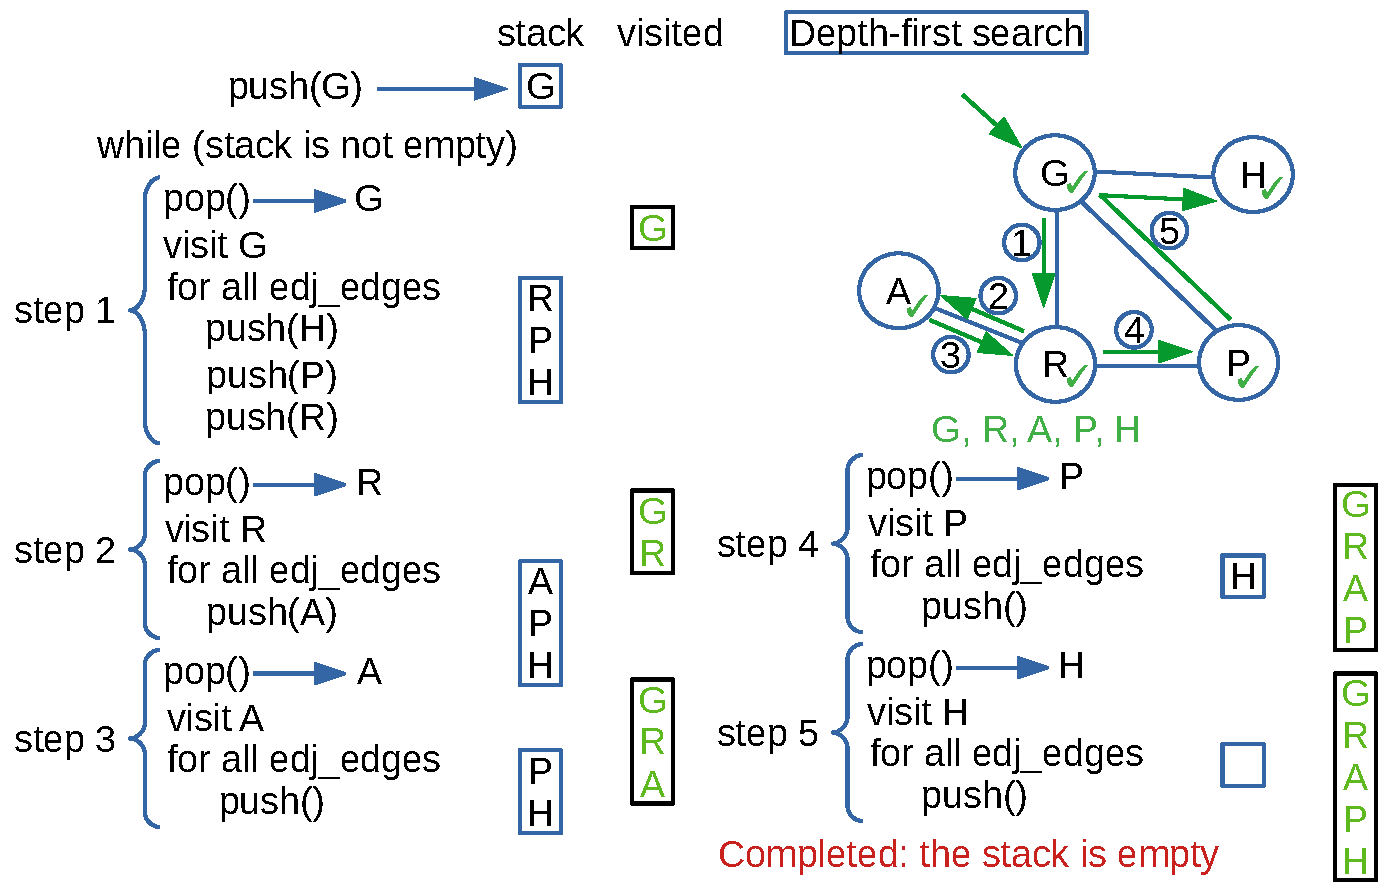
\includegraphics[scale=.6]{chapters/appendix/images/appendixgraphs/graphsappendix_1.pdf}
		\caption[Depth-first search example.]{Depth-first search example.}
		\label{graphappendix_1}
	\end{center}
\end{figure}

\section{Breadth-first search}
In the following there are the pesudocode, the python implementation, and an example of execution of the breadth-first search on a graph.

\begin{algorithm}[H]
	\DontPrintSemicolon
	\LinesNumbered
  	\SetKwFunction{FBreadthFirstSearch}{Breadth-first-search}
  	\SetKwProg{Fn}{Function}{:}{}
  	\Fn{\FBreadthFirstSearch{$graph$, $vertex$}}{
		q $\leftarrow$ \textbf{empty queue}\;
		visit(vertex)\;
		q.enqueue(vertex)\;
		\While{\normalfont{\textbf{not} q.isEmpty()}}{
			vertex $\leftarrow$ s.dequeue()\;
			\For{\normalfont{all adjacent nodes adj\textunderscore vertices to vertex}}{
				\If{\normalfont{adj\textunderscore \textbf{not} visited}}{
					visit(adj\textunderscore vertices)\;
					q.enqueue(adj\textunderscore vertices)\;
				}
			}
		}  	
  	}
\caption{Breadth-first search pseudocode.}
\end{algorithm}

\begin{lstlisting}[firstnumber=1, caption={Breadth-first search implementation on graphs.}]
		
class Graph():
	...
	
	def breadth_first_search(self, start_node):
		ret_list = [start_node]
		start_node.visited = True
		edges_out = [e for e in start_node.edges
					 if e.node_to.value != start_node.value]
		for e in edges_out:
			if not edge.node.visited:
				ret_list.extend(
					depth_first_search_recursive(
						
	
\end{lstlisting}

\begin{figure}[H]
	\begin{center}
		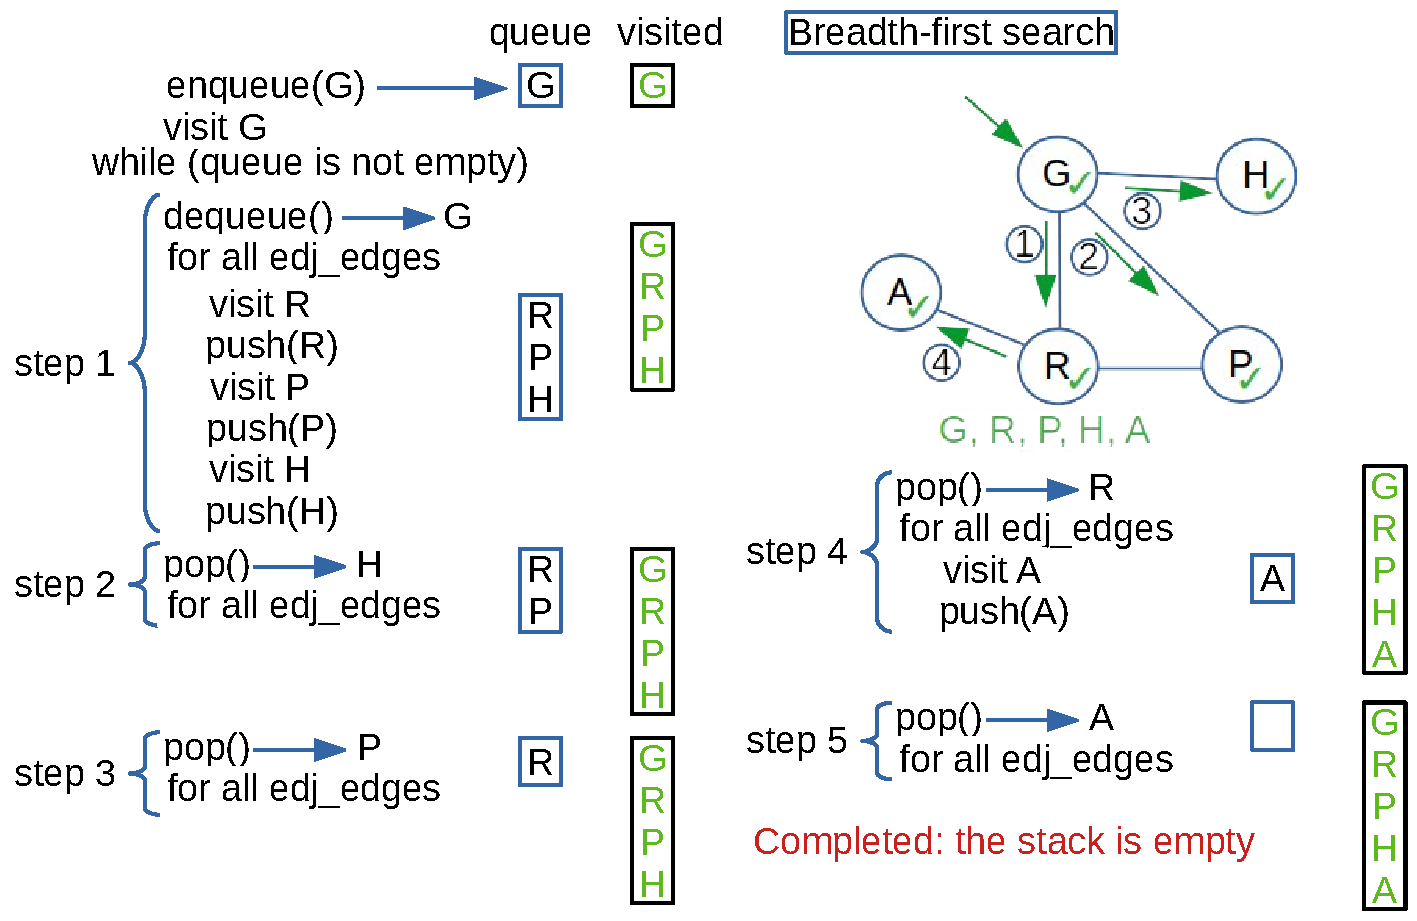
\includegraphics[scale=.6]{chapters/appendix/images/appendixgraphs/graphsappendix_2.pdf}
		\caption[Breadth-first search example.]{Breadth-first search example.}
		\label{graphappendix_2}
	\end{center}
\end{figure}

\chapter{Dijkstra's Algorithm Implementation}
\label{dijkstraimplementation}
As described in the section \ref{sec:dijkstra} the Dijkstra's algorithm is a greedy algorithm that find the optimal solution by finding the optimal solution at each step. The implementation of the Dijkstra's algorithm is based on priority queue.

For describing how the algorithm works we use the following table. At every step a new raw is added, and at the first one the table looks like the following:

\begin{table}[H]
\centering
\begin{tabular}{ l | c | c | c | c | c }
    selected vertex & 2 & 3 & 4 & 5 & 6 \\
    \hline
    4 & 50 & 45 & \mybox[rounded corners=6pt, line width=1pt, draw=red, fill=yellow!25]{mycol}{10} & \(\infty\) & \(\infty\)
\end{tabular}
\end{table}

All the nodes are listed as columns, and all the distances from the node 1 to all the others are reported in the table. The nodes 5 and 6 do not have any directed link to the node 1, then their distance is infinity. Once listed all the distances the node with the lowest one is selected: at the first step it is the node 4.

For second step all the distances of the adjacent nodes to 4 (in this case only for node 5) are updated except for the ones previously selected as the lowest. Once updated all the distances the process is repeated again, and the node with the lowest one is chosen (node 5 in this case).

\begin{table}[H]
\centering
\begin{tabular}{ l | c | c | c | c | c }
    selected vertex & 2 & 3 & 4 & 5 & 6 \\
    \hline
    4 & 50 & 45 & \mybox[rounded corners=6pt, line width=1pt, draw=black, fill=green!25]{mycol}{10} & \(\infty\) & \(\infty\) \\
    \hline
    5 & 50 & 45 & \mybox[rounded corners=6pt, line width=1pt, draw=black, fill=green!25]{mycol}{10} & \mybox[rounded corners=6pt, line width=1pt, draw=red, fill=yellow!25]{mycol}{25} & \(\infty\)
\end{tabular}
\end{table}

The process is repeated again: all the distances of the nodes adjacent to 5 are updated (in this case only the distance to node 2 is updated as the relaxation condition is fulfilled (\(25+20=45 < 50\))). At this step we have two nodes a the same distance. In this case the choice is free and one of them can be chosen indifferently. 

\begin{table}[H]
\centering
\begin{tabular}{ l | c | c | c | c | c }
    selected vertex & 2 & 3 & 4 & 5 & 6 \\
    \hline
    4 & 50 & 45 & \mybox[rounded corners=6pt, line width=1pt, draw=black, fill=green!25]{mycol}{10} & \(\infty\) & \(\infty\) \\
    \hline
    5 & 50 & 45 & \mybox[rounded corners=6pt, line width=1pt, draw=black, fill=green!25]{mycol}{10} & \mybox[rounded corners=6pt, line width=1pt, draw=black, fill=green!25]{mycol}{25} & \(\infty\) \\
    \hline
    2 & \mybox[rounded corners=6pt, line width=1pt, draw=red, fill=yellow!25]{mycol}{45} & 45 & \mybox[rounded corners=6pt, line width=1pt, draw=black, fill=green!25]{mycol}{10} & \mybox[rounded corners=6pt, line width=1pt, draw=black, fill=green!25]{mycol}{25} & \(\infty\)
\end{tabular}
\end{table}

The same process is repeated again. In this case there is also a connection from node 3 to node 5, but the node 5 has been already visited and then its weight will not be updated. Moreover, even if the weight is updated the weight would be higher and the relaxation condition would not be fulfilled.

\begin{table}[H]
\centering
\begin{tabular}{ l | c | c | c | c | c }
    selected vertex & 2 & 3 & 4 & 5 & 6 \\
    \hline
    4 & 50 & 45 & \mybox[rounded corners=6pt, line width=1pt, draw=black, fill=green!25]{mycol}{10} & \(\infty\) & \(\infty\) \\
    \hline
    5 & 50 & 45 & \mybox[rounded corners=6pt, line width=1pt, draw=black, fill=green!25]{mycol}{10} & \mybox[rounded corners=6pt, line width=1pt, draw=black, fill=green!25]{mycol}{25} & \(\infty\) \\
    \hline
    2 & \mybox[rounded corners=6pt, line width=1pt, draw=black, fill=green!25]{mycol}{45} & 45 & \mybox[rounded corners=6pt, line width=1pt, draw=black, fill=green!25]{mycol}{10} & \mybox[rounded corners=6pt, line width=1pt, draw=black, fill=green!25]{mycol}{25} & \(\infty\) \\
    \hline
    3 & \mybox[rounded corners=6pt, line width=1pt, draw=black, fill=green!25]{mycol}{45} & \mybox[rounded corners=6pt, line width=1pt, draw=red, fill=yellow!25]{mycol}{45} & \mybox[rounded corners=6pt, line width=1pt, draw=black, fill=green!25]{mycol}{10} & \mybox[rounded corners=6pt, line width=1pt, draw=black, fill=green!25]{mycol}{25} & \(\infty\)
\end{tabular}
\end{table}

The last step is to check the last node. The node 6 is not checked and it has an infinity distance. The node 6 can not be reached, and then the distance will be always infinity.

\begin{table}[H]
\centering
\begin{tabular}{ l | c | c | c | c | c }
    selected vertex & 2 & 3 & 4 & 5 & 6 \\
    \hline
    4 & 50 & 45 & \mybox[rounded corners=6pt, line width=1pt, draw=black, fill=green!25]{mycol}{10} & \(\infty\) & \(\infty\) \\
    \hline
    5 & 50 & 45 & \mybox[rounded corners=6pt, line width=1pt, draw=black, fill=green!25]{mycol}{10} & \mybox[rounded corners=6pt, line width=1pt, draw=black, fill=green!25]{mycol}{25} & \(\infty\) \\
    \hline
    2 & \mybox[rounded corners=6pt, line width=1pt, draw=black, fill=green!25]{mycol}{45} & 45 & \mybox[rounded corners=6pt, line width=1pt, draw=black, fill=green!25]{mycol}{10} & \mybox[rounded corners=6pt, line width=1pt, draw=black, fill=green!25]{mycol}{25} & \(\infty\) \\
    \hline
    3 & \mybox[rounded corners=6pt, line width=1pt, draw=black, fill=green!25]{mycol}{45} & \mybox[rounded corners=6pt, line width=1pt, draw=black, fill=green!25]{mycol}{45} & \mybox[rounded corners=6pt, line width=1pt, draw=black, fill=green!25]{mycol}{10} & \mybox[rounded corners=6pt, line width=1pt, draw=black, fill=green!25]{mycol}{25} & \(\infty\)
\end{tabular}
\end{table}